\begin{frame}
  \frametitle{X.509 PKI: Web of Trust}
  \vskip -1cm
  \begin{block}{}
    \begin{figure}
      \centering
      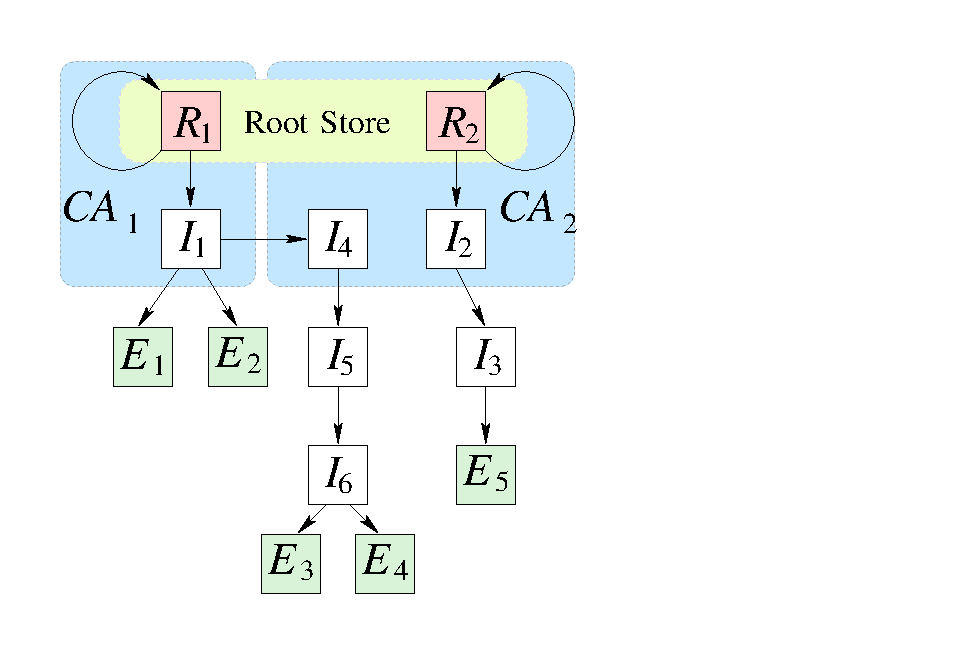
\includegraphics[scale=.7]{figures/x509tree-simplified.pdf}
    \end{figure}
  \end{block}
  \vskip -.7cm
  \begin{block}{\centering All CAs are created equal. Break one CA, break everything.}\end{block}
\end{frame}

\begin{frame}[fragile]
  \frametitle{Case study: DigiNotar}
\vskip -.8cm
    \begin{figure}
    \centering
     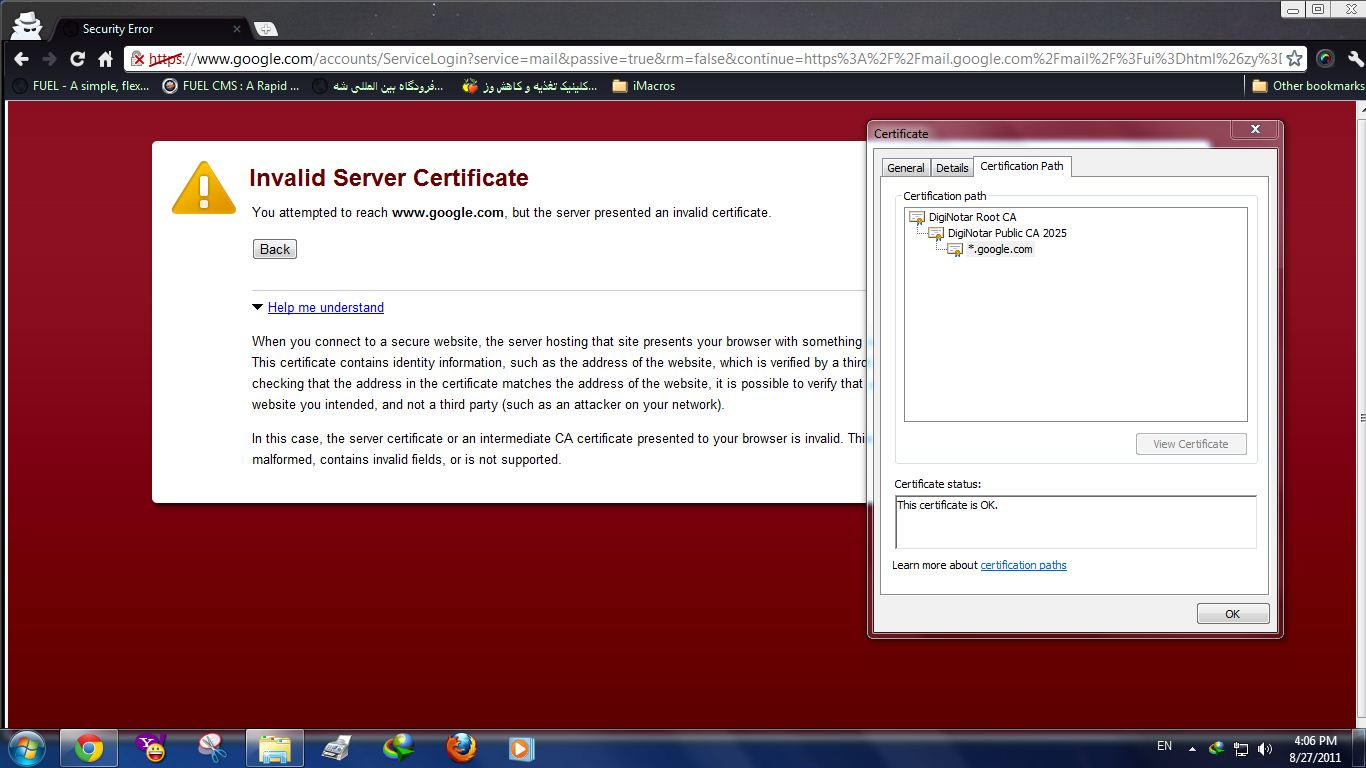
\includegraphics[scale=.37]{figures/gmail_iran.jpg}
    \end{figure}
\end{frame}

\begin{frame}
\frametitle{Crossbear: Hunting the MitM}
\begin{block}{This is \textit{not} a proposal to strengthen X.509.}\end{block}
\begin{block}{Crossbear: a tool to gather \textit{hard data}.}
  \begin{itemize}
    \item Raise reliable data about MitM \textit{in the wild}
    \item \textit{How often} do MitM attacks occur?
    \item \textit{Where} are the attackers located?
    \item \textit{Who} are the attackers?
  \end{itemize}
\end{block}
\begin{block}{Method: Combine notary principle, tracing and centralised reporting and analysis.}\end{block}
\end{frame}

%%% Local Variables:
%%% mode: latex
%%% TeX-master: "folien"
%%% End:
